\documentclass{bioinfo}
\copyrightyear{2014}
\pubyear{2014}

\usepackage{listings}

\begin{document}
\firstpage{1}

\title[short Title]{Adding versatility to Galaxy with the Dockerized integration of IPython}
\author[Sample \textit{et~al}]{Eric Rasche\,$^{2}$, Torsten Houwaart\,$^{1}$, John Chilton\,$^{3}$, Rolf Backofen\,$^{1}$ and Bj\"orn A. Gr\"uning \,$^{1}$\,\footnote{to whom correspondence should be addressed}}
\address{$^{1}$Bioinformatics Group, Department of Computer Science, University of Freiburg\\
$^{2}$Center for Phage Technology, Texas A\&M University\\
$^{3}$Department of Biochemistry and Molecular Biology, Penn State University}


\history{Received on XXXXX; revised on XXXXX; accepted on XXXXX}

\editor{Associate Editor: XXXXXXX}

\maketitle

\begin{abstract}

\section{Summary:}
The Galaxy Tool Shed enables easy installation, dependency management, and updates of tools in the Galaxy ecosystem. 
However, if tools are not available in the Galaxy Tool Shed, a Galaxy administrator often cannot help a user directly. 
This forces the user to download their data and exit the Galaxy environment to perform further analysis. The integration of 
IPython in Galaxy allows for analysis of data within the Galaxy framework with the full versatility of Python and its 
scientific libraries. This bridges the gap between users with programming experience and Galaxy by adding the flexibility 
of quickly prototyping solutions to problems and doing data analysis, while staying within the context of the Galaxy 
framework and retaining the large toolset already available. IPython is executed in a Docker container which is 
invoked and terminated automatically. This design provides a secure framework for the user and the Galaxy system.


\section{Availability and implementation:}
The integration of IPython in Galaxy was accomplished via the Galaxy Interactive Environment Framework. 
IPython Notebook security is provided by isolation within a Docker container. The IPython IE
is now part of Galaxy and is freely available under the MIT License. The Docker image is hosted on Docker Hub under bgruening/docker-ipython-notebook and is used automatically by the IE.

\section{Contact:} \href{bjoern.gruening@gmail.com}{bjoern.gruening@gmail.com}
\end{abstract}

\section{Introduction}


The Galaxy platform \citep{Blank2010,Giardine2005,Goecks2010} has made advanced bioinformatics software accessible
to life scientists for many years. Galaxy has a default set of analysis tools and can be extended with additional locally produced tools, or by using the community driven collections of tools available from the Galaxy Tool Shed
\citep{Blankenberg2014}. This approach to extending Galaxy is sufficient in most cases, but a more flexible tool allowing 
for more tailored analysis may be needed.
In this work the IPython Galaxy project is introduced. This project extends the Galaxy framework with an interface to an
IPython \citep{Perez2007} instance running inside a Docker container.
IPython provides a web service which allows for a graphical and interactive way to compute and visualize data, 
extensible through publicly available Python libraries. The IPython instance is run within a Docker container, 
isolating the written code from the rest of the system and providing security for both the user and the Galaxy instance. Finally, by providing and encouraging a route for arbitrary data analysis to be accomplished within the Galaxy framework, 
IPython notebooks allow for saved and embedded logs of analysis, furthering the ultimate goal of research reproducibility.



\begin{methods}
\section{Methods}

IPython is integrated as an Interactive Environment (IE) in Galaxy. The program flow is illustrated in 
figure~\ref{fig:diagram}. An Interactive Environment primarily consists of a python Mako template file and some
associated configuration data. The IE configuration allows for additional security constraints which is useful
for production instances. Password authentification and encrypted data transfer via SSL are both available.
Additionally, the name of a custom Docker image can be provided in the configuration. This image will be downloaded and 
installed from the Docker Hub. The default Docker image is specially crafted for use in conjunction with the I
Python Interactive Environment and will be described in more detail later. The configuration is also responsible for providing a history dataset 
association (HDA) for the template file in order to access the data. \\
The template file is written in Mako, a Python template engine which can be used in conjunction with HTML
% RFY: Mako needs a reference
and Javascript code to generate web pages. In the first part of the template file, a configuration is generated with a password, 
an Application Programming Interface (API) key for the Docker container, and a unique port for communication. These pieces of information are stored so that Galaxy
and the Dockerized IPython web service can communicate securely, while isolated from the rest of the Galaxy instance.

Once container configuration and other preparatory work are complete, the Docker container is launched with bi-directional
access to a temporary directory containing the necessary initialization information. The container is built on top of a basic Debian Wheezy installation,
and provides an IPython server, with its dependencies and additional Python libraries such as NumPy \citep{Walt2011}, SciPy \citep{Jones2015} and Matplotlib \citep{Hunter2007}.
By providing a Docker image with a full suite of Python scientific analysis tools and libraries, users are able 
to immediately perform their analysis and calculations. Additional Python packages can be installed with Python
package managers, e.g.\ pip. The same holds for R packages. Moreover, tools that can be installed in a non-privileged user account can be added to the container on demand. 
% RFY: Same as above. Pip and R need to be referenced
The IPython notebook is then embedded inside the usual Galaxy interface and can be used to interactively program in a variety of programming languages.
Having abstracted the chosen container into a site-specific configuration option, Galaxy instances with different use cases
and needs can provide Docker images to their users with appropriate tool suites.\\
During Docker container startup, a cron job is launched, monitoring whether the IPython service
is still being used by checking the network traffic. If the page with the IPython notebook is closed, the
Docker process automatically terminates itself. Within the IPython Notebook, 
two important custom functions are defined which enable the
user to load data from the history or store data to the Galaxy history using the Galaxy API \citep{Sloggett2013}.
The \textit{get} function expects one parameter with the identifier of the dataset which corresponds to the number
of the dataset in the history. The \textit{put} function automatically builds a connection to the host
Galaxy instance and uploads a specified file from inside the Docker container to the user's
history. The flexibility is obvious: any dataset can be
loaded into the notebook, datasets can be combined or modified, and the results can be written back to the history.
The entire traffic occures between the Galaxy host and the IPython Docker container without the need for the user to upload or download data to the client. \\
Notebooks can be saved back to the Galaxy history at any time. Once a notebook is part of a history 
it can be inspected as any other Galaxy dataset. 
Additionaly, it can be reused to start a new IPython instance reloading the saved notebook. 
It should be stressed that this functionality ensures the reproducibility of data analysis and is therefore an essential
feature of the IPython Interactive Environment.


\section{Use Cases}
The Galaxy IPython integration is not designed to restrict the user. Rather, the intention is to enable
reproducible research with best practices. IPython is not bound to any programming language 
and offers, with it's modular approach, many additional features through a growing community.

Moreover, the IPython Notebook provides direct access to a pre-configured
BioBlend object, allowing the user to make API calls as necessary. Having access to the Galaxy programming interface
can be invaluable for running batch analyses, launching multiple workflows over numerous datasets, etc. 
% this needs a small rewrite I guess
%In order to respect security, information necessary
%to accomplish this is stored outside of notebooks and available inside as static variables. The user is able to use
%\texttt{API\_KEY} without displaying their API key, which is essential if the user intends to publish their notebook as
%part of their research effort.

Merging/Combining? the flexibility of IPython and the powerful Galaxy infrastructure creates an research environment
with a tremendous amout of freedom and possibilities. Given that we would like to showcase only one simple
example to demonstrate how easy data manipulation with Galaxy and IPython is. 

Heretofore, a Galaxy user wanting to transform and plot a specific column of a dataset and
get the result in a file of the Scalable Vector Graphics (SVG) format to do further image manipulation,
would have to download the dataset, a time-consuming process depending on file size and their internet
connection. In addition, the user would have to record the commands used for plotting, if reproducibility was desired.
With the use of the IPython IE, the user can easily load datasets inside the IPython Notebook.
There the data can be manipulated with a fully functional programming shell, plots generated,
and finally datasets and notebooks stored and published.
This workflow reduces the input time and effort required on the end user significantly and keeps everything in one place.

\lstset{language=python,
morekeywords={put, get}
}
\begin{lstlisting}[frame=single,caption={Plotting example},label=code:import]]
from matplotlib import pyplot as p
filename = get(57)
p.plotfile(filename,delimiter='\t',cols=(0,12))
p.savefig("col12.svg")
put("col12.svg")
\end{lstlisting}

In code listing~\ref{code:import}, the dataset which has the ID 57 in the Galaxy history is loaded 
into the IPython notebook inside the plotfile method of a matplolib.pyplot object. 
The 13th column of this file is plotted against the first column and the
resulting plot is stored as a SVG file. The \textit{put} command copies the image into the Galaxy history, creating a persistent
downloadable and sharable Galaxy object.


%
%visualization plugin how implemented used because ease of integration
%
%config files provides history dataset association And general variables calls mako
%
%mako file mainly prepares a docker container with a configuration file and a notebook access url (with a specific docker port)
%invokes the docker container with
%
%API
%hist.id
%paswd
%conf.yaml
%
%mako template
%invoke docker
%command
%/import/configfile in docker
%runs ipython -> HTML object
%docker monitors tcp connections as cron job -> docker cleans up and kills itself
%
%IPython
%%predefined functions: get(datasetNr.) copy dataset into docker ocntainer .. example?
%%knows history_id
%put (filename,type)
%
%
%docker image what's in it
%
%put/get
%
%API key

\begin{figure}[!tpb]
\centerline{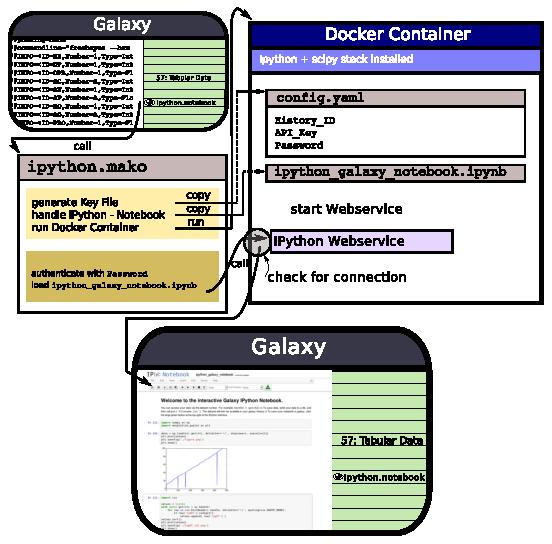
\includegraphics{diagram.pdf}}
\caption{Program Flow when using IPython IE. The IPython IE is divided into two parts;
The first part generates initialization information and an IPython notebook, the second part launches a container
from a specific Docker image. IPython and its dependencies are installed in this Docker container as well as additional Python
libraries. The configuration file and the IPython notebook are copied to the container and the IPython service is started.
The second part of the IE template now generates a connection to the web service provided by the Docker container.
For self cleaning, the container also checks whether a connection to the host exists, enabling self termination 
if no longer in use.}
\label{fig:diagram}
\end{figure}


\end{methods}

\section{Conclusion}
The IPython Interactive Environment adds versatility to Galaxy by embedding a Python shell in a secure and easy-to-install manner.
This Interactive Environment is a major shortcut for a user with programming experience who cannot wait for a specific tool to
be implemented in Galaxy or who needs more control to manipulate data. The potential applications of this IE are extensive.
The example explained above is just a glimpse of what could be done with the full scientific Python stack in conjunction with R and a Unix Shell.
The major security concern of giving users access a potentially exploitable tool like IPython, 
has been resolved by running the IPython web service inside a Docker container. This 
isolates IE users from the rest of the Galaxy server, protecting the system and keeping sensitive data secure.
%Users are additionally restricted by limits which administrators have placed on Docker containers,
%preventing single users from launching denial of service attacks through over-use of memory/CPU cycles.
The user can interact with the Galaxy instance via the two predefined functions \textit{put} and \textit{get} 
which essentially define the exchange between the container and the Galaxy instance.
Storing IPython notebooks in Galaxy histories enables sharing with other users. 
This way users with no programming experience can benefit from notebooks developed by users with programming experience.
With these possibilities a consistent and reproducible data analysis is simple and encouraged. 


\section*{Acknowledgement}
We would like to thank the Galaxy team and the Galaxy community for being so inspiring and helpful. 
Additionally we would like to thank Dr.~Ryland Young, of the Center for Phage Technology at Texas A\&M University, 
and Cameron R. Smith, for editing help.

\paragraph{Funding\textcolon} The project was supported by the German Research Foundation (DFG-grant SFB 992/1).

\bibliographystyle{natbib}
%\bibliographystyle{achemnat}
%\bibliographystyle{plainnat}
%\bibliographystyle{abbrv}
%\bibliographystyle{bioinformatics}
%
%\bibliographystyle{plain}
%
%\bibliography{Document}


\begin{thebibliography}{}
\bibitem[Blankenberg {\it et~al}., 2010]{Blank2010}
Blankenberg, A. {\it et~al}., (2010) Galaxy: a web-based genome analysis tool for experimentalists. \textit{Curr. Protoc. Mol. Biol.},  {\bf Chapter 19}, Unit 19.10.1-21.

\bibitem[Giardine {\it et~al}., 2005]{Giardine2005}
Giardine, D. {\it et~al}., (2005) Galaxy: a platform for interactive large-scale genome analysis. \textit{Genome Res.},  {\bf 15}, 1451-1455.

\bibitem[Goecks {\it et~al}., 2010]{Goecks2010}
Goecks, J. {\it et~al}., (2005) Galaxy: a comprehensive approach for supporting accessible, reproducible, and transparent computational research in the life sciences. \textit{Genome Biol.},  {\bf 11}, R86.

\bibitem[P\'erez {\it et~al}., 2007]{Perez2007}
P\'erez, F. {\it et~al}., (2007) IPython: A System for Interactive Scientific Computing. \textit{Comput. Sci. Eng.}, {\bf 9}, 21-29.

\bibitem[Sloggett {\it et~al}., 2013]{Sloggett2013}
Sloggett, C. {\it et~al}., (2013) BioBlend: automating pipeline analyses within Galaxy and CloudMan. \textit{Bioinformatics}, {\bf 29}, 1685-1686.

\bibitem[Blankenberg {\it et~al}., 2014]{Blankenberg2014}
Blankenberg, A. {\it et~al}., (2014) Dissemination of scientific software with Galaxy ToolShed. \textit{Genome Biol.}, {\bf 15}, 403.

\bibitem[van der Walt {\it et~al}., 2011]{Walt2011}
van der Walt, S. {\it et~al}., (2011) The NumPy Array: A Structure for Efficient Numerical Computation \textit{Comput. Sci. Eng.}, {\bf 13}, 22-30.

\bibitem[Jones {\it et~al}., 2015]{Jones2015}
Jones, E. {\it et~al}., (2015) SciPy: Open Source Scientific Tools for Python  \textit{online}, http://www.scipy.org

\bibitem[Hunter, 2007]{Hunter2007}
Hunter, J. , (2007) Matplotlib: A 2D Graphics Environment \textit{Comput. Sci. Eng.}, {\bf 9}, 90-95.



\end{thebibliography}
\end{document}
